% !TEX root = ../main.tex

\section{Current state of affairs and future work}
\label{now}

In previously cited survey study \cite{Sermpezis2018}, most of the network operators (71\%) answered that they have not deployed RPKI as a proactive defense mechanism in their networks \ref{fig:usagerpki}; very few (12\%) use the full functionality of RPKI (Route Origin Authorization -- ROA and Route Origin Validation -- ROV). ROA is used by 15\% of networks.

\begin{figure}[ht]
 \begin{center}
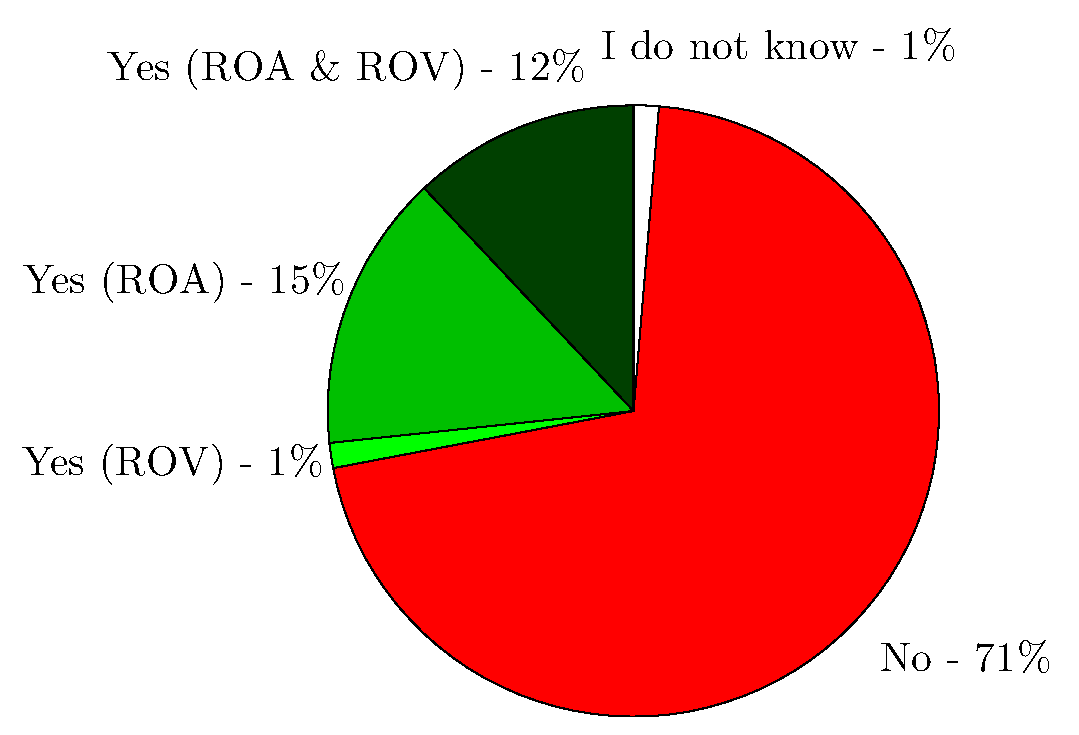
\includegraphics[width = 0.8\linewidth]{./fig/fig_survey_use_RPKI}
 \end{center}
 \caption{Usage of RPKI based on survey by \cite{Sermpezis2018}} \label{fig:usagerpki}
\end{figure}

However, these number seems to be changing, as cam be seen on \ref{fig:rpki-rov} and \ref{fig:rpki-roa}.

\begin{figure}[ht]
	\begin{center}
   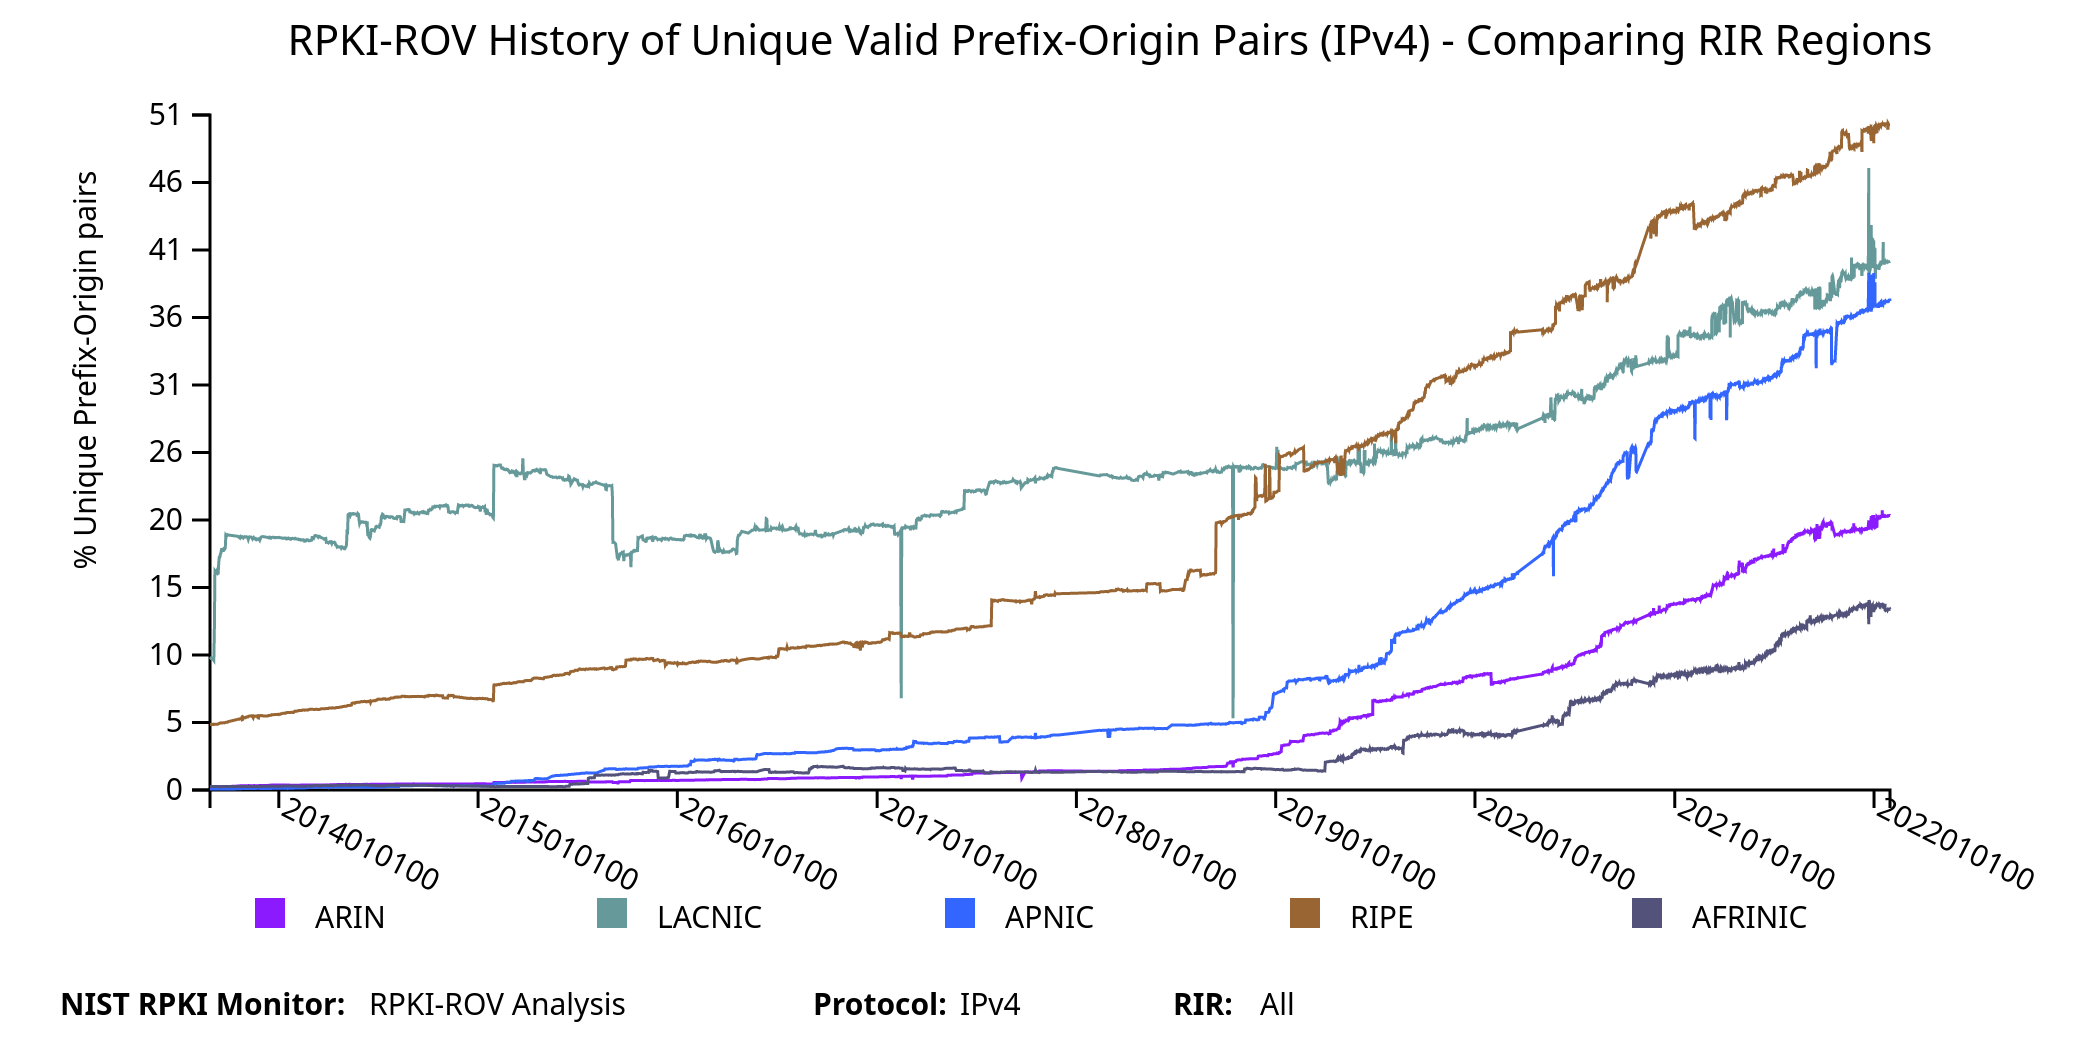
\includegraphics[width = 1\linewidth]{./img/RPKIROV_20220130.png}
	\end{center}
	\caption{A percent of the total count unique announced Prefix-Origin pairs with prefixes in the corresponding RIR. Source: NIST RPKI Monitor \label{fig:rpki-rov}}
\end{figure}
\begin{figure}[ht]
	\begin{center}
   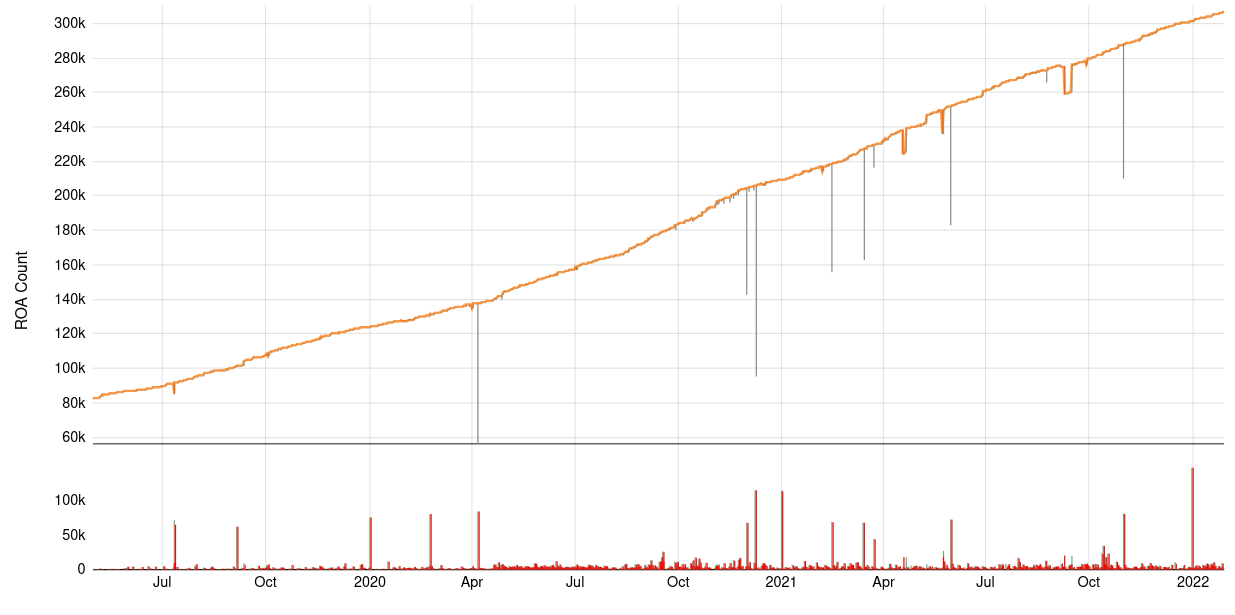
\includegraphics[width = 1\linewidth]{./img/ROA-history.png}
	\end{center}
	\caption{Total count of ROA over time. Source: Cloudflare RPKI Portal\label{fig:rpki-roa}}
\end{figure}
\subsection{Slow adoption}
\label{now:slow}



\subsubsection{Lack of awareness}
TODO

MANRS is doing a great job\cite{Robachevsky2020}

\subsubsection{Technical difficulties}
Researches in \cite{Sermpezis2018} points that
\textquote{deployment lags mainly due to RPKI's limited adoption and little security benefits, but also due to the increased CAPEX and OPEX costs, and increased complexity and processing overhead associated with the protocol mechanisms. Therefore, about 60\% of the operators  resort to other mechanisms and practical defenses to protect their networks against BGP hijacks.} For detailed breakdown of adoption slowiness causes, see fig. \ref{fig:notrpkireasons}.


 \begin{figure}[h]
 	\begin{center}
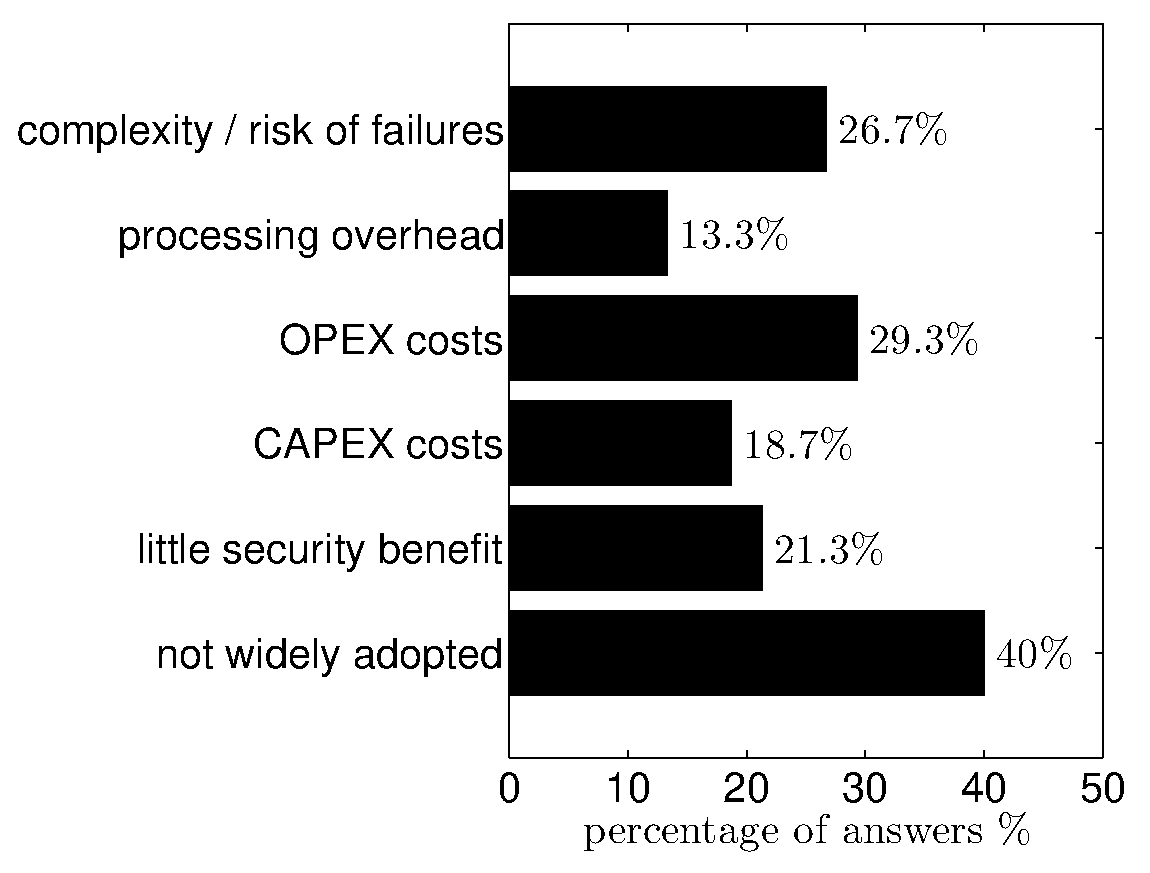
\includegraphics[width = 1\linewidth]{./fig/fig_survey_reasons_rpki}
 	\end{center}
 	\caption{Main reasons not using RPKI based on survey by \cite{Sermpezis2018}} \label{fig:notrpkireasons}
 \end{figure}

\subsubsection{Legal issues}
Widespread RPKI adoption may be limited due to specific status on ARIN's terms and conditions for RPKI repository.
Third parties who wish to validate BGP routes had to agree \emph{Relying Party Agreement}.
As a result, most RP validating software does not come with ARIN TAL embedded by default.


This has a direct effect on ARIN members in North America -- Route Origin Validation on ARIN AS' has been significantly lower. Almost 80\% of those AS engaging in ROV omit the ARIN TAL, has been proofed by \cite{CartwrightCox2018}.

In the beginning of 2019, the gap between ARIN's ROA only grew. This state of affairs was criticized in work \cite{Yoo2019}, but researchers presented 6 solutions.
However, in late 2019 the RPA was changed \cite{Curran2019}.
The change \textquote{was intended to accommodate and overcome claimed barriers to RPKI adoption} and distribution in machine readable formats has been approved. In author opinion, although the change is in a good direction, a desired state of good and simple configuration is still obstructed.


\subsubsection{Low RPKI deployment penetration factor among CDNs}
Content Delivery Networks have crucial function in the global Internet, providing usually heavy content to the user in a fast, reliable and cheap manner. It is estimated that over a half of all web traffic is served over CDNs, therefore securing this segment is prominent in the global scale.

Researchers in \cite{Waehlisch2014} investigated some among most important CDNs: Akamai, Amazon, Cdnetworks, Chinacache, Cloudflare, Cotendo, Edgecast, Highwinds, Instart, Internap, Limelight, Mirrorimage, Netdna, Simplecdn, and Yottaa.

\begin{displayquote}
(By the reverse IP lookup, they -- note ed.) discovered 199 ASes operated by these CDNs. From these, we find only four entries in the RPKI. These four prefixes are owned by Internap and are tied to three origin ASes.  One might mistakenly think that Internap has therefore engaged widely with RPKI. However, Internap operates at least 41 ASes, the bulk of which are not secured via RPKI. No other CDN has made any deployment. Thus, these CDNs do not actively participate in the creation of RPKI attestation objects.
\end{displayquote}

To combat this low adoption progress, {MANRS} consortium has launched dedicated \emph{program for CDN and Cloud Providers} on April 2020. As of December 3, 2020 the program has 14 members \cite{Siddiqui2020}. One of the mandatory Actions is \textquote{Fostering RPKI as the primary technology for validation of routing information on a global scale}, while \textquote{Improving consistency of route validation based on route objects published in an IRR}.


%%%%%%%%%%%%%%

\subsection{RPKI infrastructure work}
\label{now:future}


\subsubsection{rsync depreciation}
RPKI repositories and Relying Party software performing RPKI Validation will use the RPKI Repository Delta Protocol (RRDP) [RFC8182]
\cite{ietf-sidrops-deprecate-rsync-00}
\subsubsection{}

\subsection{New approach on Path Validation}
\label{now:future:path}
aha BGP AS\_PATH validatin


ASPA? \cite{ietf-sidrops-aspa-profile-04} \cite{ietf-sidrops-aspa-verification-06}


\cite{Borchert2016} implementing BGP-SRx

\cite{Junjie2020}


%%%%%%%%%%%%%%%%%%

\subsection{Caveats}
\label{now:caveats}
\subsubsection{RPKI MaxLength parameter}
subprefix hijack
\cite{ietf-sidrops-rpkimaxlen-05}

\subsubsection{Unilateral IP space takedowns}

\cite{Shrishak2020}

\subsubsection{MOAS}
colision clash conflict
\cite{Zhao2001}
